\documentclass[nojss]{jss}\usepackage[]{graphicx}\usepackage[]{color}
%% maxwidth is the original width if it is less than linewidth
%% otherwise use linewidth (to make sure the graphics do not exceed the margin)
\makeatletter
\def\maxwidth{ %
  \ifdim\Gin@nat@width>\linewidth
    \linewidth
  \else
    \Gin@nat@width
  \fi
}
\makeatother

\definecolor{fgcolor}{rgb}{0.345, 0.345, 0.345}
\newcommand{\hlnum}[1]{\textcolor[rgb]{0.686,0.059,0.569}{#1}}%
\newcommand{\hlstr}[1]{\textcolor[rgb]{0.192,0.494,0.8}{#1}}%
\newcommand{\hlcom}[1]{\textcolor[rgb]{0.678,0.584,0.686}{\textit{#1}}}%
\newcommand{\hlopt}[1]{\textcolor[rgb]{0,0,0}{#1}}%
\newcommand{\hlstd}[1]{\textcolor[rgb]{0.345,0.345,0.345}{#1}}%
\newcommand{\hlkwa}[1]{\textcolor[rgb]{0.161,0.373,0.58}{\textbf{#1}}}%
\newcommand{\hlkwb}[1]{\textcolor[rgb]{0.69,0.353,0.396}{#1}}%
\newcommand{\hlkwc}[1]{\textcolor[rgb]{0.333,0.667,0.333}{#1}}%
\newcommand{\hlkwd}[1]{\textcolor[rgb]{0.737,0.353,0.396}{\textbf{#1}}}%

\usepackage{framed}
\makeatletter
\newenvironment{kframe}{%
 \def\at@end@of@kframe{}%
 \ifinner\ifhmode%
  \def\at@end@of@kframe{\end{minipage}}%
  \begin{minipage}{\columnwidth}%
 \fi\fi%
 \def\FrameCommand##1{\hskip\@totalleftmargin \hskip-\fboxsep
 \colorbox{shadecolor}{##1}\hskip-\fboxsep
     % There is no \\@totalrightmargin, so:
     \hskip-\linewidth \hskip-\@totalleftmargin \hskip\columnwidth}%
 \MakeFramed {\advance\hsize-\width
   \@totalleftmargin\z@ \linewidth\hsize
   \@setminipage}}%
 {\par\unskip\endMakeFramed%
 \at@end@of@kframe}
\makeatother

\definecolor{shadecolor}{rgb}{.97, .97, .97}
\definecolor{messagecolor}{rgb}{0, 0, 0}
\definecolor{warningcolor}{rgb}{1, 0, 1}
\definecolor{errorcolor}{rgb}{1, 0, 0}
\newenvironment{knitrout}{}{} % an empty environment to be redefined in TeX

\usepackage{alltt}
\usepackage{url}
\usepackage[sc]{mathpazo}
\usepackage{geometry}
\geometry{verbose,tmargin=2.5cm,bmargin=2.5cm,lmargin=2.5cm,rmargin=2.5cm}
\setcounter{secnumdepth}{2}
\setcounter{tocdepth}{2}
\usepackage{breakurl}
\usepackage{hyperref}
\usepackage[ruled, vlined]{algorithm2e}
\usepackage{mathtools}
\usepackage{draftwatermark}
\usepackage{float}
\usepackage{placeins}
\usepackage{mathrsfs}
\usepackage{multirow}
%% \usepackage{mathbbm}
\DeclareMathOperator{\sgn}{sgn}
\DeclareMathOperator*{\argmax}{\arg\!\max}



\title{\bf faoswsFlag:A package to manage flag aggregation}

\author{Michael. C. J. Kao\\ Food and Agriculture Organization \\ of
  the United Nations}

\Plainauthor{Michael. C. J. Kao} 

\Plaintitle{faoswsFlag:A package to manage flag aggregation}

\Shorttitle{Flag module}

\Abstract{ 

  This short documentation is intended to explain how observation
  flags are aggregated in the ESS Statistical Working System.

}

\Keywords{meta data, flag aggregation}
\Plainkeywords{meta data, flag aggregation}

\Address{
  Michael. C. J. Kao\\
  Economics and Social Statistics Division (ESS)\\
  Economic and Social Development Department (ES)\\
  Food and Agriculture Organization of the United Nations (FAO)\\
  Viale delle Terme di Caracalla 00153 Rome, Italy\\
  E-mail: \email{michael.kao@fao.org}\\
  URL: \url{https://github.com/mkao006/sws_imputation}
}
\IfFileExists{upquote.sty}{\usepackage{upquote}}{}
\begin{document}





Lets start by loading the required library into R.

\begin{knitrout}
\definecolor{shadecolor}{rgb}{0.969, 0.969, 0.969}\color{fgcolor}\begin{kframe}
\begin{alltt}
\hlcom{## Load the required libraries}
\hlkwd{library}\hlstd{(faoswsFlag)}
\hlkwd{library}\hlstd{(ggplot2)}
\end{alltt}
\end{kframe}
\end{knitrout}

Since the introduction of the new statistical working system, the old
symb which reprents how the data was collected and computed is split
into two separate flags. The first, an observation flag which is a
description of the observation status, whether it be official,
estimates or imputed value. While on the other hand, the methodology
flag contains information of how it is collected or computed. It can
be from survey, questionnaire or it can be obtained as a balance or
estimated through statistical methodology.

This paper concerns mainly the observation flag, where the data
originated and the information content it is associated with.

Shown below is the corresponding table for the observation flags as of
\today{} outlined in Annex 5 of FAO Statistical Standards:

\begin{table}[h!]
  \begin{center}
    \caption{Description of the Observation flag}
    \begin{tabular}{|c|p{12cm}|}
      \hline
      Flags & Description\\
      \hline
      <blank> & Official Figure\\
      E & Estimates\\
      I & Imputed\\
      M & Missing\\
      T & Unofficial figure\\
      \hline
    \end{tabular}
  \end{center}  
\end{table}

One of the main goal for this package is to provide a consistent
framework for handling multiple flags and flag aggregation.

In order to compute aggregation of flags, one must convert the symbol
into a numerical type. The way how this is handled is based on the
amount of information quantity and the reliability of the observation
status.

Information obtained from reliable source should have a high
information content and thus should be converted to a high value,
while data estimated or derived should have a lower information vice
versa.

Shown below is the default weights table for the new statistical
working system which comes along with the package.

\begin{knitrout}
\definecolor{shadecolor}{rgb}{0.969, 0.969, 0.969}\color{fgcolor}\begin{kframe}
\begin{alltt}
\hlcom{## Printed here is the default flag conversion table shipped with the}
\hlcom{## package.}
\hlstd{faoswsFlagTable}
\end{alltt}
\begin{verbatim}
##   flagObservationStatus flagObservationWeights
## 1                                         1.00
## 2                     T                   0.80
## 3                     E                   0.75
## 4                     I                   0.50
## 5                     M                   0.00
\end{verbatim}
\end{kframe}
\end{knitrout}

From this table, we have assigned 1 to official figure while 0 to
missing values. Albeit the arbitrary selection of the values, it
provides a rank of the information content which is what we need in
order to compute flag aggregation.

Take the computation of yield for example, the value is computed based
on production and area harvested which may come from different
sources. Thus, when we compute a derived statistic which is unobserved
such as yield it is important to reflecte the information content
which associated with this derivative. For a set of aggregation, the
minimum of the set is taken as the final observation flag.

Lets say we have a production value of 30,000 recorded from official
survey (), while the area harvested was collected from an unofficial
private data base (T). As shown in the following code, the resulting
flag for yield should return (T) to reflect the lower information
content of the unofficial figure.


\begin{knitrout}
\definecolor{shadecolor}{rgb}{0.969, 0.969, 0.969}\color{fgcolor}\begin{kframe}
\begin{alltt}
\hlcom{## The function works just like sum(), with an optional arguement for}
\hlcom{## the flag table to be used.}
\hlkwd{aggregateObservationFlag}\hlstd{(}\hlstr{""}\hlstd{,} \hlstr{"T"}\hlstd{,} \hlkwc{flagTable} \hlstd{= faoswsFlagTable)}
\end{alltt}
\begin{verbatim}
## [1] "T"
\end{verbatim}
\end{kframe}
\end{knitrout}

\begin{knitrout}
\definecolor{shadecolor}{rgb}{0.969, 0.969, 0.969}\color{fgcolor}\begin{kframe}
\begin{alltt}
\hlcom{## Aggregation of multiple flag}

\hlcom{## Simulate flag for production}
\hlstd{simulatedProductionFlag} \hlkwb{=}
    \hlstd{faoswsFlagTable[}\hlkwd{sample}\hlstd{(}\hlnum{1}\hlopt{:}\hlkwd{NROW}\hlstd{(faoswsFlagTable),} \hlnum{10}\hlstd{,} \hlkwc{replace} \hlstd{=} \hlnum{TRUE}\hlstd{),}
                    \hlstr{"flagObservationStatus"}\hlstd{]}
\hlstd{simulatedProductionFlag}
\end{alltt}
\begin{verbatim}
##  [1] "T" "E" "E" "T" "I" "I" ""  "E" "I" "I"
\end{verbatim}
\begin{alltt}
\hlcom{## Simulated flag for area harvested}
\hlstd{simulatedAreaFlag} \hlkwb{=}
    \hlstd{faoswsFlagTable[}\hlkwd{sample}\hlstd{(}\hlnum{1}\hlopt{:}\hlkwd{NROW}\hlstd{(faoswsFlagTable),} \hlnum{10}\hlstd{,} \hlkwc{replace} \hlstd{=} \hlnum{TRUE}\hlstd{),}
                    \hlstr{"flagObservationStatus"}\hlstd{]}
\hlstd{simulatedAreaFlag}
\end{alltt}
\begin{verbatim}
##  [1] "E" "E" "I" "M" ""  ""  ""  "M" ""  "M"
\end{verbatim}
\begin{alltt}
\hlcom{## Now compute the aggregation of flag}
\hlkwd{aggregateObservationFlag}\hlstd{(simulatedProductionFlag, simulatedAreaFlag,}
                         \hlkwc{flagTable} \hlstd{= faoswsFlagTable)}
\end{alltt}
\begin{verbatim}
##  [1] "E" "E" "I" "M" "I" "I" ""  "M" "I" "M"
\end{verbatim}
\end{kframe}
\end{knitrout}


Currently, the flags are chosen as arbitrary mainly to preserve a rank
order based on expert judgement. Nevertheless, this information can be
estimated from the data and history of the flag. This is currently
under investigation, yet the idea is simple. First, we take official
figure as the golden benchmark, then we calculate the deviation of
each observation which has a value collected priorly with a different
flag. This will allow us to compute the relative error of flags and in
turn to estimate the information content.


Associating a value with its meta data has significant advantages, as
it provides information about the data which can be used in further
analysis or improvements of modelling. For example, instead of fitting
a linear regression by treating all observation equally, we can
estimate a weighted regression which gives more weight to data which
are of higher reliability. 


The following artificial example illustrates how accounting for the
information source can result in a better fit and incorporate poor
data quality. The artificial data starts in 1990 and ends in 2014,
with all the observation collected as official figure except for
2009. For illustrative purpose, the value in 2009 was imputed by a
poor algorithm and can be seen in the graph as an outlier. The
illustration shows how accounting for the outlier through the use of
meta data can result in more robust model fitting than as treating all
data have the same information quality.

The black dots are the original data, with the red line being the
linear regression treating all observation equally while the blue line
incorporates the information quality through the flags. We can see
that by accounting for the source, the fit of the blue line is less
affected by the outlier generated by the poor imputation algorithm.

\begin{knitrout}
\definecolor{shadecolor}{rgb}{0.969, 0.969, 0.969}\color{fgcolor}\begin{kframe}
\begin{alltt}
\hlcom{## Simuate a data set which has a single point that was imputed badly }
\hlcom{## but still used for later analysis.}
\hlstd{x} \hlkwb{=} \hlnum{1990}\hlopt{:}\hlnum{2014}
\hlstd{y} \hlkwb{=} \hlnum{100} \hlopt{+} \hlnum{10} \hlopt{*} \hlstd{(x} \hlopt{-} \hlnum{1989}\hlstd{)} \hlopt{+} \hlkwd{rnorm}\hlstd{(}\hlkwd{length}\hlstd{(x),} \hlkwc{sd} \hlstd{=} \hlnum{20}\hlstd{)}
\hlstd{f} \hlkwb{=} \hlkwd{rep}\hlstd{(}\hlstr{""}\hlstd{,} \hlkwd{length}\hlstd{(x))}
\hlstd{y[}\hlnum{20}\hlstd{]} \hlkwb{=} \hlstd{y[}\hlnum{20}\hlstd{]} \hlopt{+} \hlnum{500}
\hlstd{f[}\hlnum{20}\hlstd{]} \hlkwb{=} \hlstr{"I"}
\hlstd{simulated.df} \hlkwb{=} \hlkwd{data.frame}\hlstd{(}\hlkwc{year} \hlstd{= x,} \hlkwc{simulatedProduction} \hlstd{= y,} \hlkwc{flag} \hlstd{= f)}

\hlcom{## Plot the data and show the two different fit when accounting for the }
\hlcom{## source and quality of information.}
\hlkwd{ggplot}\hlstd{(}\hlkwc{data} \hlstd{= simulated.df,}
       \hlkwd{aes}\hlstd{(}\hlkwc{x} \hlstd{= year,} \hlkwc{y} \hlstd{= simulatedProduction))} \hlopt{+}
    \hlkwd{geom_point}\hlstd{()} \hlopt{+}
    \hlkwd{geom_smooth}\hlstd{(}\hlkwc{method} \hlstd{=} \hlstr{"lm"}\hlstd{,} \hlkwc{formula} \hlstd{= y} \hlopt{~} \hlstd{x,}
                \hlkwc{data} \hlstd{= simulated.df,} \hlkwc{se} \hlstd{=} \hlnum{FALSE}\hlstd{,} \hlkwc{col} \hlstd{=} \hlstr{"red"}\hlstd{)} \hlopt{+}
    \hlkwd{geom_smooth}\hlstd{(}\hlkwc{method} \hlstd{=} \hlstr{"lm"}\hlstd{,} \hlkwc{formula} \hlstd{= y} \hlopt{~} \hlstd{x,}
                \hlkwd{aes}\hlstd{(}\hlkwc{weight} \hlstd{=} \hlkwd{flag2weight}\hlstd{(flag)),}
                \hlkwc{data} \hlstd{= simulated.df,} \hlkwc{se} \hlstd{=} \hlnum{FALSE}\hlstd{)}
\end{alltt}
\end{kframe}

{\centering 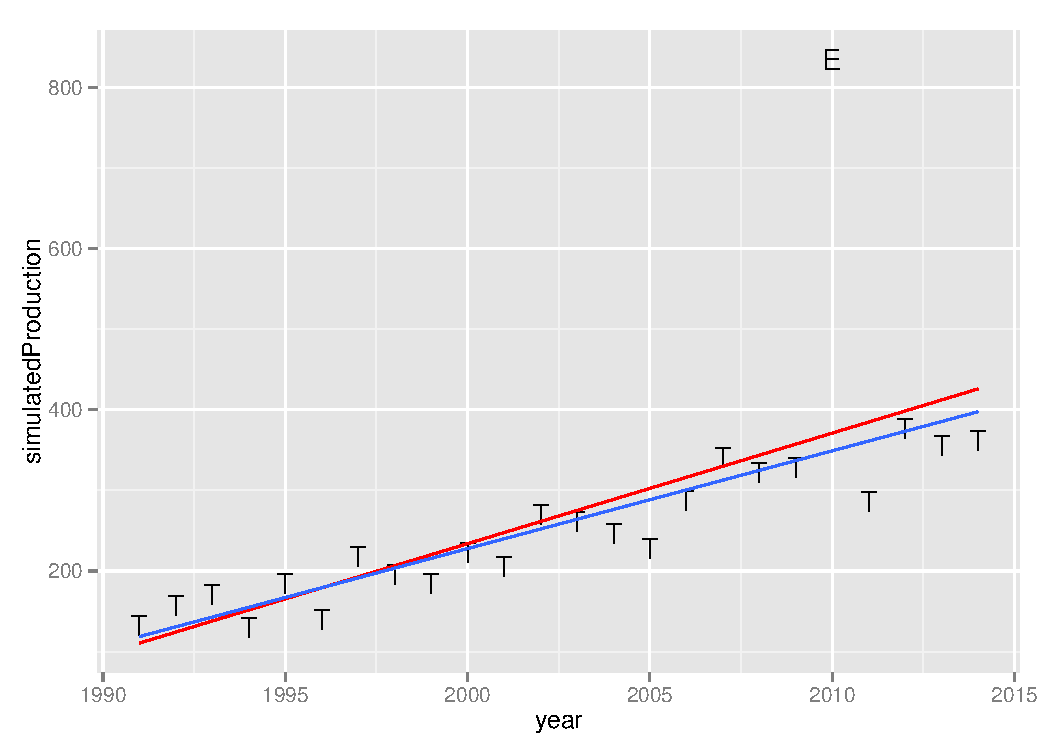
\includegraphics[width=\maxwidth]{figure/simulated-example} 

}



\end{knitrout}







\end{document}
